\documentclass[a4paper, 9pt, landscape]{extarticle}
\usepackage[scaled=0.92]{helvet}
\usepackage{multicol}
\usepackage{calc}
\usepackage{ifthen}
\usepackage[landscape]{geometry}
%\usepackage{hyperref}

\usepackage{newtxtext} 

%for strikeout
\usepackage{ulem}

%For editing parbox
\usepackage[table]{xcolor}
%For editing itemise margins, reduce iterm separaion and list separation
\usepackage{enumitem}
% For math
\usepackage{amsmath,amsthm,amsfonts,amssymb}

%For pictures / figures
\usepackage{color,graphicx,overpic}
\graphicspath{ {./images/} }

%\usepackage{newtxtext} 
%\usepackage{amssymb}
%\usepackage[table]{xcolor}
%\usepackage{vwcol}
%\usepackage{tikz}
%\usepackage{wrapfig}
%\usepackage{makecell}

\pdfinfo{
  /Title (CS4222.pdf)
  /Creator (Ger Teck)
  /Author (Ger Teck)
  /Subject ()
  /Keywords (tex)}

%% Margins for PAPER

% This sets page margins to .5 inch if using letter paper, and to 1cm
% if using A4 paper. (This probably isn't strictly necessary.)
% If using another size paper, use default 1cm margins.
% \ifthenelse{\lengthtest { \paperwidth = 11in}}
%	{ \geometry{top=.3in,left=.3in,right=.3in,bottom=.3in} }
%	{\ifthenelse{ \lengthtest{ \paperwidth = 297mm}}
%		{\geometry{top=1cm,left=1cm,right=1cm,bottom=1cm} }
%		{\geometry{top=1cm,left=1cm,right=1cm,bottom=1cm} }
%	}

%% Margins for A4 PAPER
\geometry{top=0.5cm,left=0.5cm,right=0.5cm,bottom=0.5cm}

% Turn off header and footer
\pagestyle{empty}

% for tight centres (less spacing)
\newenvironment{tightcenter}{%
  \setlength\topsep{0pt}
  \setlength\parskip{0pt}
  \begin{center}
}{%
  \end{center}
}

% Redefine section commands to use less space
\makeatletter
\renewcommand{\section}{\@startsection{section}{1}{0mm}%
                                {-1ex plus -.5ex minus -.2ex}%
                                {0.5ex plus .2ex}%x
                                {\normalfont\large\bfseries}}
\renewcommand{\subsection}{\@startsection{subsection}{2}{0mm}%
                                {-1explus -.5ex minus -.2ex}%
                                {0.5ex plus .2ex}%
                                {\normalfont\normalsize\bfseries}}
\renewcommand{\subsubsection}{\@startsection{subsubsection}{3}{0mm}%
                                {-1ex plus -.5ex minus -.2ex}%
                                {1ex plus .2ex}%
                                {\normalfont\small\bfseries}}

% 4. Subsubsection acts as Paragraph (Level 4) - BLOCK STYLE
\renewcommand{\subsubsection}{\@startsection{paragraph}{4}{0mm}%
                                {-1ex plus -.5ex minus -.2ex}% Space above
                                {0.5ex plus .2ex}% POSITIVE value = Block (New line)
                                {\normalfont\footnotesize\bfseries}} % Smaller font

% change font
%\renewcommand{\familydefault}{\sfdefault}
%\renewcommand\rmdefault{\sfdefault}
\makeatother

% Define BibTeX command
\def\BibTeX{{\rm B\kern-.05em{\sc i\kern-.025em b}\kern-.08em
    T\kern-.1667em\lower.7ex\hbox{E}\kern-.125emX}}

% Don't print section numbers
\setcounter{secnumdepth}{0}

\setlength{\parindent}{0pt}
\setlength{\parskip}{0pt plus 0.5ex}

%% this changes all items (enumerate and itemize, reduce margins)
\setlength{\leftmargini}{0.5cm}
\setlength{\leftmarginii}{0.5cm}
\setlist[itemize,1]{leftmargin=2mm,labelindent=1mm,labelsep=1mm, itemsep = 0mm, before=\justifying}
\setlist[itemize,2]{leftmargin=2mm,labelindent=0.5mm,labelsep=0.5mm, itemsep = -0.2mm, topsep=-0.2mm, before=\justifying}
%\setlist{nosep}

\usepackage[document]{ragged2e}

% -------------------------------------------------------------------------------

% START OF DOCUMENT HERE

\begin{document}
\raggedright
\footnotesize
\begin{multicols*}{3}

% multicol parameters
% These lengths are set only within the two main columns
\setlength{\columnseprule}{0pt}
\setlength{\premulticols}{1pt}
\setlength{\postmulticols}{1pt}
\setlength{\multicolsep}{2pt}
\setlength{\columnsep}{2pt}

\section{CS4222 Wireless Networking}
\centerline{AY25/26 Sem 2. github.com/gerteck}


\section{1: Introduction to Wireless Networks}
\subsection{CS4222 Course Overview}
\begin{itemize}
\item \textbf{Principles of wireless networking}: studied within the context of Internet of Things (IoT). 
\item Covers signal propagation, modulation, energy consumption estimation. Various layers of wireless networking stack (physical (PHY), MAC, networking, application). Case studies of popular wireless technologies (WiFi, Bluetooth), cellular networks, IoT.
\item \textbf{{Learning Philosophy}}: Focus on \textbf{application of concepts}, not memorization, hands-on programming with real wireless devices.
\item Use of \textbf{SensorTag} wireless embedded devices, programmed using \textbf{Contiki OS}.
\end{itemize}

\subsection{Internet of Things (IoT)}

\begin{itemize}
\item \textbf{IoT}: Network of embedded devices with sensing, computation, and communication. Devices interact with physical world and the Internet. (E.g. smart bulbs, wearables, sensors, beacons).
\item \textbf{4 Core Tasks of an IoT Device}: Computation and Storage, Sensing and Actuation, Power Management, Wireless Networking.
\item \textbf{Typical IoT Architecture}: Sensors and actuators at the edge (ADC: Analog to Digital Converter). Embedded processor for computation (MCU: Microcontroller Unit). Wireless interface for communication. Backend/cloud for storage and analytics.
\end{itemize}

\centerline{
\includegraphics[width = 0.8\linewidth]{architecture}}

\begin{itemize}
\item \textbf{ARM}: ARM (Advanced RISC Machines) is a low-power RISC (reduced instruction set computer) processor architecture (and ecosystem) widely used in embedded and IoT devices due to its energy efficiency, small footprint, and suitability for battery-powered wireless systems. 
\item \textbf{ARM Holdings Ltd.} provides the Instruction Set Architecture (ISA), CPU core designs (small part of the chip), tools etc. and licenses to semiconductor companies (e.g., Qualcomm, Apple, Samsung) to design and manufacture their own ARM-based chips.
\item \textbf{Prevalence}: Billions of embedded devices already deployed, ARM shipped 4.4B Cortex-M processors in Q4 2020.
\item \textbf{Energy Trend}: Computation energy cost decreasing rapidly. Wireless communication remains energy-expensive
Energy efficiency is a key design constraint
\end{itemize}


\subsection{History of Wireless Communication}
\begin{itemize}
  \item \textbf{Early Wireless Milestones}: 1880: Bell and Tainter invent photophone (sound over light), 1893: Tesla demonstrates wireless radio communication, 1896--1899: Marconi achieves km-scale radio transmission, 1901: Transatlantic wireless transmission
  \item \textbf{Broadcasting Evolution}: 1906: First AM radio audio broadcast. 1935: Frequency Modulation (FM)
  1920s--30s: Radio stations worldwide. 1980s: Digital Audio Broadcasting (DAB)
  \item \textbf{Television Broadcasting}: 1923: First wireless TV transmission. 1941: NTSC standard (US). 1962: Telstar satellite. 1967: PAL standard (Analog TV standard in many countries). 2000s: Digital TV transition
  \item \textbf{WiFi Timeline}: 1985: ISM band opened for unlicensed use. 1997: IEEE 802.11 standard. 1999: 802.11a/b and WiFi Alliance. 1999: First consumer WiFi (Apple iBook)
\end{itemize}
\centerline{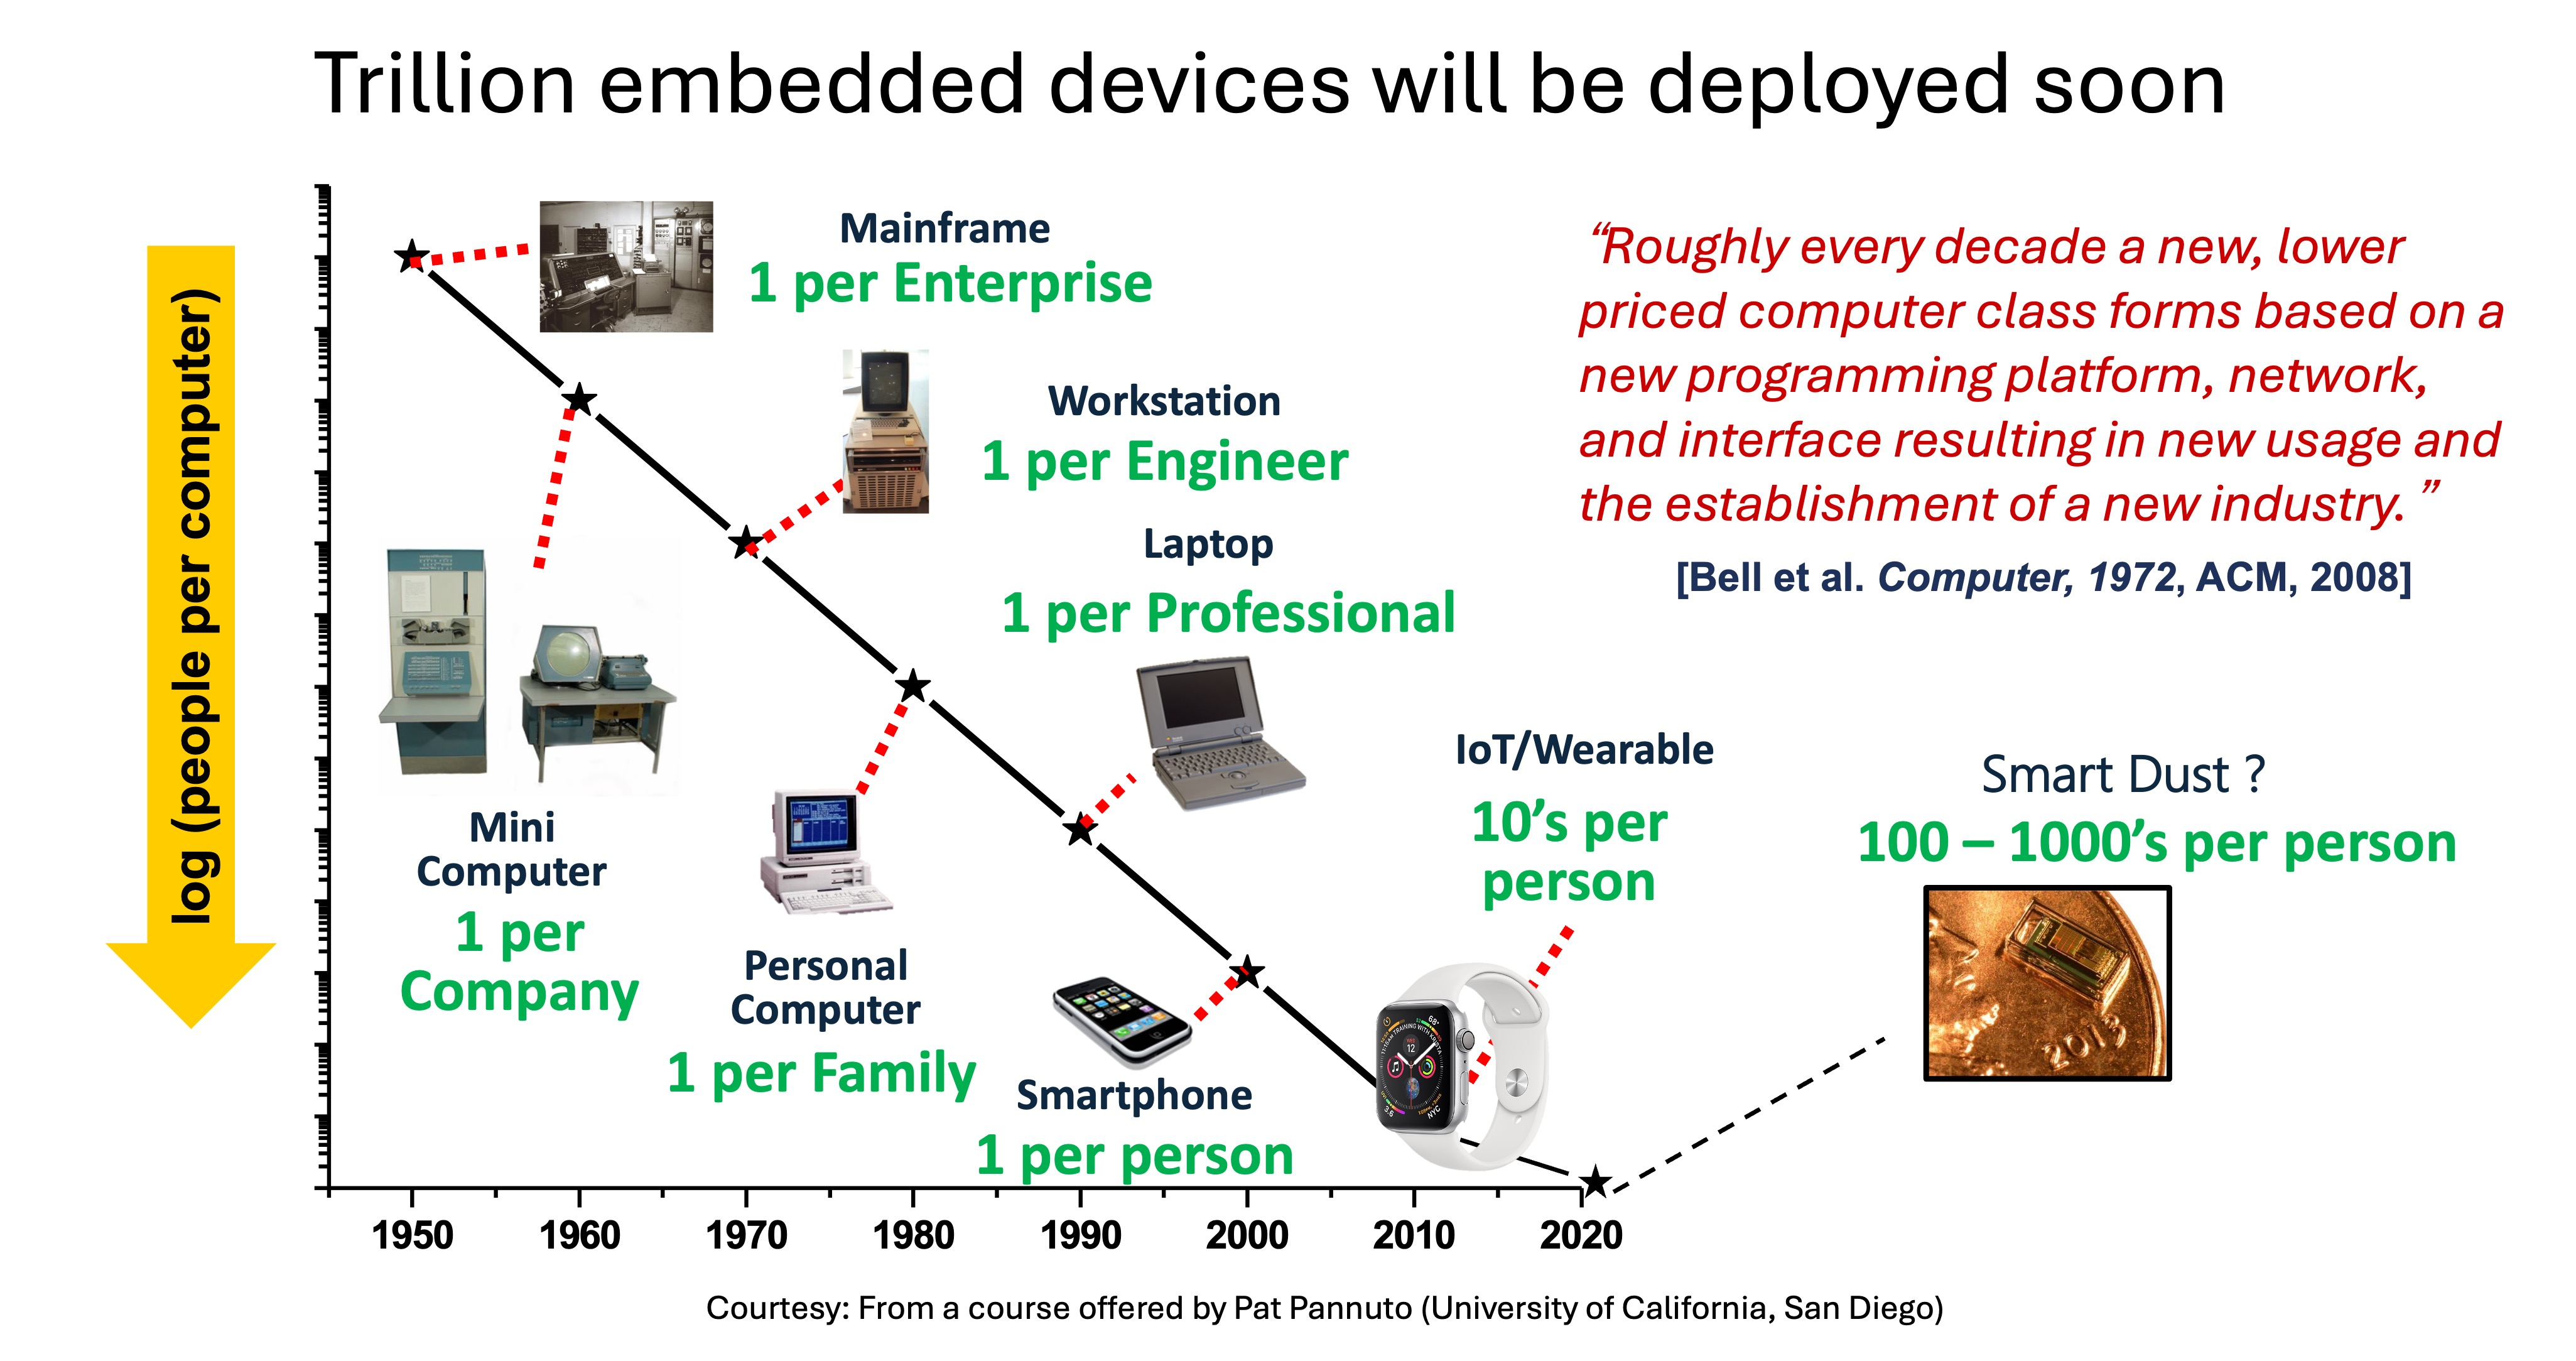
\includegraphics[width = 0.8\linewidth]{history}}

\subsection{Basics of Wireless Communication}
\begin{itemize}
\item \textbf{Radio}: Latin \textit{radius} (ray). Communication using EM waves from 3 Hz to 300 GHz. Frequency bands collectively called \textbf{radio spectrum}.
\item \textbf{Radio Transceivers}: Enable transmission and reception of EM waves. Key component of an \textbf{antenna}, present in WiFi, Bluetooth, smartphones, IoT devices
\item \textbf{Electromagnetic (EM) Waves}: EM waves consist of oscillating electric and magnetic fields,f, Frequency: cycles per second (Hz). Period inversely proportional to frequency.
\item \textbf{Wavelength ($\lambda$)}: $\lambda = \frac{c}{f}$. (Since $v = fx$) Speed of light: $c = 3 \times 10^8$ m/s.
\item \textbf{Example Wavelengths}: 3 kHz $\Rightarrow$ $\lambda \approx 100$ km, 100 MHz (FM) $\Rightarrow$ $\lambda = 3$ m.
\item 2.4 GHz (WiFi) $\Rightarrow$ $\lambda = 0.125$, 300 GHz $\Rightarrow$ $\lambda = 1$ mm
\item \textbf{Radio Terminology}: Radio technology implies transmitting and receiving EM waves using of frequency 3Hz to 300GHz. EM waves at these frequencies also called radio waves, frequency bands also called radio spectrum.
\end{itemize}
\centerline{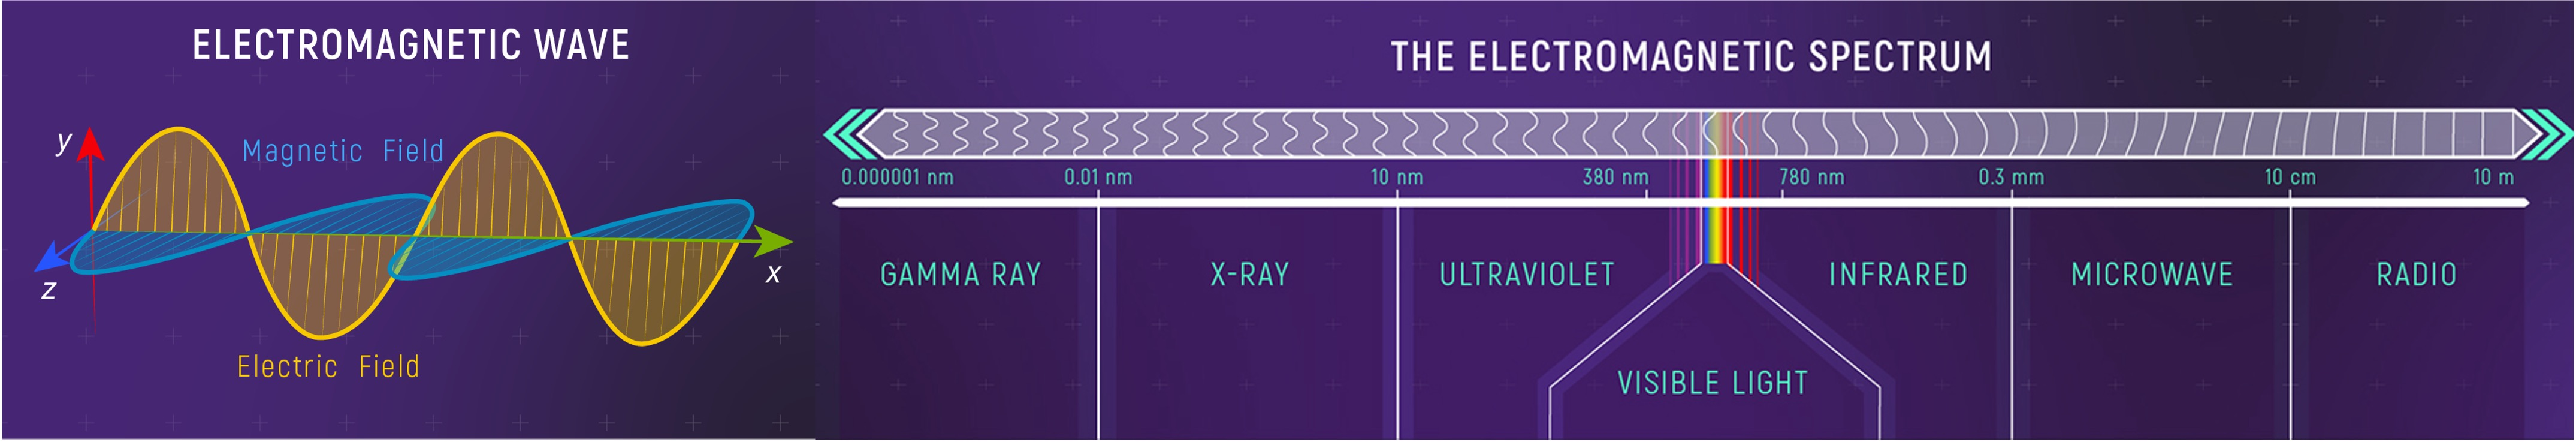
\includegraphics[width = 1\linewidth]{waveSpectrum}}

\subsection{Radio Spectrum}
\begin{itemize}
\item \textbf{Radio Waves}: Modern communcation systems relies on radio waves, longest wavelength in EM spectrum (3 Hz to 300 GHz).
\item \textbf{Radio Wave Characteristics}: \\
\textbf{Strength/Power}: energy contained in the radio wave.\\
\textbf{Frequency}: rate of periodic variation between electric and magnetic fields. \\
\textbf{Bandwidth}: range of frequencies occupied by the signal.\\
\textbf{Polarization}: orientation of the electric field - circular, elliptical, linear.\\
\textbf{Modulation}: method of encoding information onto the carrier wave.
\end{itemize}
\centerline{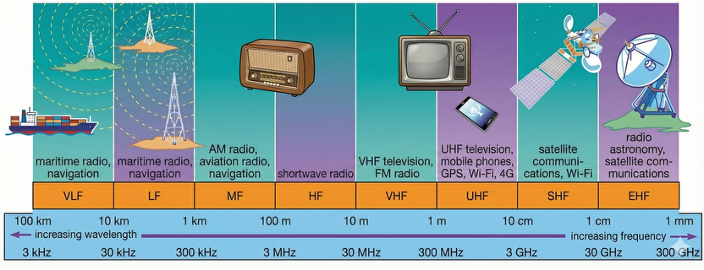
\includegraphics[width = 0.8\linewidth]{radioWaves}}

\subsection{Antennas}
\begin{itemize}
  \item \textbf{Antenna}: Basically an electrical conductor or array of conductors designed to transmit, receive EM waves. (Transmit (TX): electrical energy to EM waves. Reception (RX): Opposite).
  \item \textbf{Directionality}: directional, omnidirectional (radiates equally in all directions).
  \item \textbf{Common Antenna types}: Monopole (straight rod on conductive ground plane, e.g. cars). Array (multiple elements form directional beam, e.g. radar). Parabolic (dish reflector e.g. satellite). Patch (flat element on substrate, e.g. mobile devices), loop, aperture etc. Dipole Antenna: Two conductors in opposite directions. 
  \item \textbf{Antenna Size vs Frequency}: Antenna size inversely proportional to frequency of radio wave, lower frequency requires larger antenna. This is cause antennas work by resonating with the radio waves, working efficiently when it is a significant fraction of the signal wavelength. (E.g. half-wave dipole length ($\lambda / 2$), quarter-wave monopole length ($\lambda / 4$)).
  \item Size $\propto \frac{1}{f}$: Low frequency $\Rightarrow$ very large antennas. High frequency $\Rightarrow$ compact antennas.
\end{itemize}

\subsection{Antenna Gain}
\begin{itemize}
\item \textbf{Antenna gain}: dimensionless quantity, measures ability of antenna to direct or receive radio waves in a particular direction compared to a reference. Usually measured in decibels (dB). 
\item Measure of directionality in reference to hypothetical isotropic antenna (dBi), or halfwave dipole antenna (dBd). Antennas are reciprocal (TX = RX performance)
\item \textbf{Tradeoff}: Higher gain: arrower beamwidth (more directional). Lower gain: wider beamwidth.
\item \textbf{Performance of Antenna}: Power output in given direction, compared to that produced in any direction by perfect isotropic antenna radiating same total power.
\item \textbf{Gain Formula}: $G = \frac{4\pi A_e}{\lambda^2} = \frac{4\pi f^2 A_e}{c^2}$. $A_e$: effective antenna area. Pure ratio, no units.
\item \textbf{Decibel Conversion}: $G_{\text{dBi}} = 10 \log_{10}(G)$ For calculating in decibel scale, compress ratios.
\item Antenna gain does not create energy, just concentrate energy in certain directions.
\end{itemize}


\subsection{Radio Wave Propagation Effects}
\begin{itemize}
\item \textbf{Radio Wave Propagation}: Strongly influenced by environment. Obstacles cause reflection, diffraction, scattering. Non-line-of-sight common in real deployments
\item \textbf{Practical Impacts}: Reduced communication range, Increased interference, Lower reliability
\end{itemize}











\end{multicols*}
\end{document}
